\chapter{\faust syntax}

This section describes the syntax of \faust. Figure \ref{fig:syntax} gives an overview of the various concepts and where they are defined in this section. 
%% suggestion Carlos : la figure crée une confusion entre la structure de la syntaxe et la structure de la section. Faire un autre schema!
\begin{figure}[ht!]
\centering
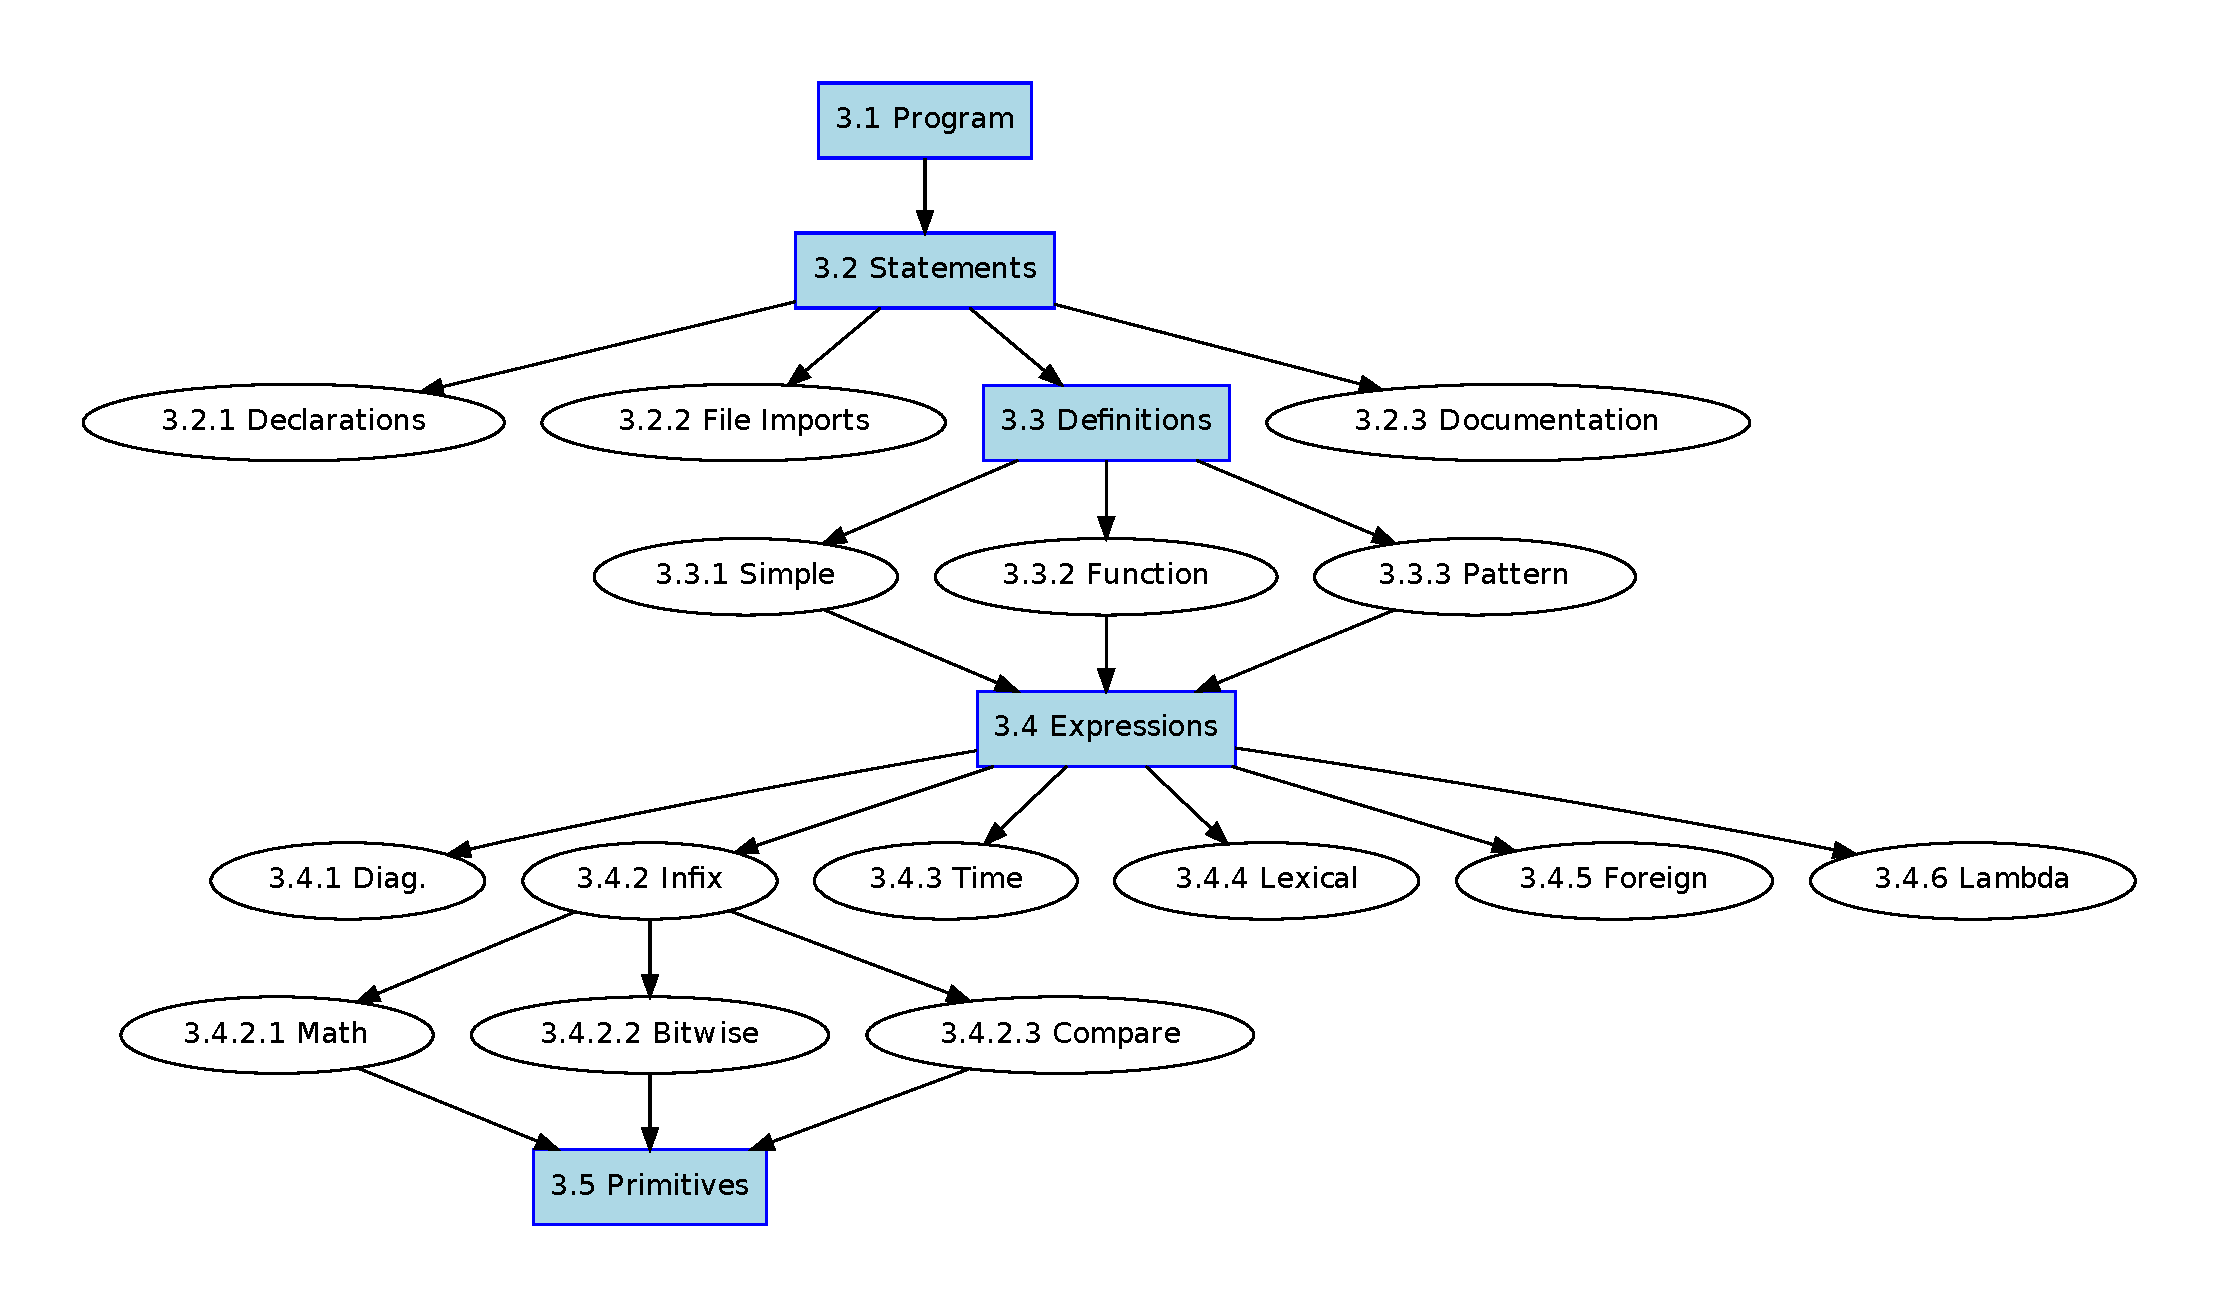
\includegraphics[scale=0.45]{illustrations/syntax-chart}
\caption{Overview of \faust syntax}
\label{fig:syntax}
\end{figure}

As we will see, \textit{definitions} and \textit{expressions} have a central role.

\section{\faust program}

A \faust program is essentially a list of \textit{statements}. These statements can be \textit{declarations}, \textit{imports}, \textit{definitions} and \textit{documentation tags}, with optional C++ style (//... and /*...*/) comments.
 
\begin{rail}
program : (statement)+;
\end{rail}

Here is a short \faust program that implements of a simple noise generator. It exhibits various kind of statements : two \textit{declarations}, an \textit{import}, a \textit{comment} and a \textit{definition}. We will see later on \textit{documentation} statements (\ref{sec:documentation}).

\begin{lstlisting}
declare name       "noise";
declare copyright  "(c)GRAME 2006";

import("music.lib");

// noise level controlled by a slider
process = noise * vslider("volume", 0, 0, 1, 0.1);
\end{lstlisting}
 
The keyword \lstinline'process' is the equivalent of \lstinline'main' in C/C++. Any \faust program, to be valid, must at least define \lstinline'process'.


\section{Statements}

The \textit{statements} of a \faust program are of four kinds : \textit{metadata declarations}, \textit{file imports},  \textit{definitions} and \textit{documentation}. All statements but documentation end with a semicolon (\lstinline';'). 
% 
% \begin{grammar}
%   <statement> ::= 
%   \begin{syntdiag}
%     \begin{stack}
%       <declaration>\\
%       <fileimport>\\
%       <definition>\\
%       <documentation>
%     \end{stack}
%   \end{syntdiag}
% \end{grammar}

\begin{rail}
statement : declaration | fileimport | definition | documentation;
\end{rail}

\subsection{Declarations}

Meta-data declarations (for example \lstinline'declare name "noise";') are optional and typically used to document a \faust project. 

% \begin{grammar}
%   <declaration> ::= 
%   \begin{syntdiag}
%     "declare" <key> <string> ";"
%   \end{syntdiag}
% \end{grammar}
% 
% \begin{grammar}
%   <key> ::= 
%     <identifier>
% \end{grammar}

\begin{rail}
declaration : "declare" key string ';';
key : identifier;
\end{rail}

Contrary to regular comments, these declarations will appear in the C++ code generated by the compiler. A good practice is to start a \faust program with some standard declarations:
\begin{lstlisting}
declare name "MyProgram";
declare author "MySelf";
declare copyright "MyCompany";
declare version "1.00";
declare license "BSD"; 
\end{lstlisting}



\subsection{Imports}

File imports allow to import definitions from other source files.  

% \begin{grammar}
%   <fileimport> ::= 
%   \begin{syntdiag}
%     "import"  "(" <filename> ")" ";"
%   \end{syntdiag}
% \end{grammar}

\begin{rail}
fileimport : "import" '(' filename ')' ';';
\end{rail}

For example \lstinline{import("math.lib");} imports the definitions of the \lstinline{math.lib} library, a set of additional mathematical functions provided as foreign functions.


\subsection{Documentation}
\label{sec:documentation}

Documentation statements are optional and typically used to control the generation of the mathematical documentation of a \faust program. This documentation system is detailed chapter \ref{chapter:mdoc}. In this section we will essentially describe the documentation statements syntax.

A documentation statement starts with an opening \lstinline'<mdoc>' tag and ends with a closing \lstinline'</mdoc>' tag. Free text content, typically in \latex format, can be placed in between these two tags. 

% \begin{grammar}
%   <documentation> ::= 
%   \begin{syntdiag}
%     "<mdoc>"     
%     \begin{stack}
%       <free text>\\
%       <equation>\\
%       <diagram>\\
%       <metadata>\\
%       <notice>\\
%       <listing>
%     \end{stack}
%     "</mdoc>"
%   \end{syntdiag}
% \end{grammar}

\begin{rail}
documentation : "<mdoc>" ((freetext|equation|diagram|metadata|notice|listing)+) "</mdoc>";
\end{rail}


Moreover, optional sub-tags can be inserted in the text content itself to require the generation, at the insertion point, of mathematical \textit{equations}, graphical \textit{block-diagrams}, \faust source code \textit{listing} and explanation \textit{notice}.

% \begin{grammar}
%   <equation> ::= 
%   \begin{syntdiag}
%     "<equation>" <expression> "</equation>"
%   \end{syntdiag}
% \end{grammar}

\begin{rail}
equation : "<equation>" expression "</equation>";
\end{rail}

The generation of the mathematical equations of a \faust expression can be requested by placing this expression between an opening \lstinline'<equation>' and a closing \lstinline'</equation>' tag. The expression is evaluated within the lexical context of the \faust program.

% \begin{grammar}
%   <diagram> ::= 
%   \begin{syntdiag}
%     "<diagram>" <expression> "</diagram>"
%   \end{syntdiag}
% \end{grammar}

\begin{rail}
diagram : "<diagram>" expression "</diagram>";
\end{rail}

Similarly, the generation of the graphical block-diagram of a \faust expression can be requested by placing this expression between an opening \lstinline'<diagram>' and a closing \lstinline'</diagram>' tag. The expression is evaluated within the lexical context of the \faust program.

% \begin{grammar}
%   <diagram> ::= 
%   \begin{syntdiag}
%     "<metadata>" <keyword> "</metadata>"
%   \end{syntdiag}
% \end{grammar}


\begin{rail}
metadata : "<metadata>" keyword "</metadata>";
\end{rail}


The \lstinline'<metadata>' tags allow to reference \faust metadatas (cf. declarations), calling the corresponding keyword.

% \begin{grammar}
%   <notice> ::= 
%   \begin{syntdiag}
%     "<notice />"
%   \end{syntdiag}
% \end{grammar}

\begin{rail}
notice : "<notice />";
\end{rail}

The \lstinline'<notice />' empty-element tag is used to generate the conventions used in the mathematical equations.
% 
% \begin{grammar}
%   <listing> ::= 
%   \begin{syntdiag}
%     "<listing " 
%     \begin{stack}
%       \\
%       \begin{rep}
%         <listingattribute>
%       \end{rep}
%     \end{stack}
%     " />"
%   \end{syntdiag}
% \end{grammar}

\begin{rail}
listing : "<listing" (listingattribute*) " />";
listingattribute : ("mdoctags" | "dependencies" | "distributed") "=" ('"true"' | '"false"');
\end{rail}


% \begin{grammar}
%   <listingattribute> ::= 
%   \begin{syntdiag}
%     \begin{stack}
%       "mdoctags" \\
%       "dependencies" \\
%       "distributed"
%     \end{stack}
%     "=" "\""
%     \begin{stack}
%       "true" \\ "false"
%     \end{stack}
%     "\""
%   \end{syntdiag}
% \end{grammar}

The \lstinline'<listing />' empty-element tag is used to generate the listing of the \faust program. Its three attributes \lstinline'mdoctags', \lstinline'dependencies' and \lstinline'distributed' enable or disable respectively \lstinline'<mdoc>' tags, other files dependencies and distribution of interleaved faust code between \lstinline'<mdoc>' sections.


\section{Definitions}

A \textit{definition} associates an identifier with an expression it stands for. 

Definitions are essentially a convenient shortcut avoiding to type long expressions. During compilation, more precisely during the evaluation stage, identifiers are replaced by their definitions. It is therefore always equivalent to use an identifier or directly its definition. Please note that multiple definitions of a same identifier are not allowed, unless it is a pattern matching based definition.

\subsection{Simple Definitions}

The syntax of a simple definition is:

\begin{rail}
definition  : identifier '=' expression ';';
\end{rail} 

For example here is the definition of \lstinline'random', a simple pseudo-random number generator:

\begin{lstlisting}
 random = +(12345) ~ *(1103515245);
\end{lstlisting}


\subsection{Function Definitions}

Definitions with formal parameters correspond to functions definitions.

\begin{rail}
definition  : identifier '(' (parameter + ',')  ')' '=' expression ';';
\end{rail} 

For example the definition of \lstinline'linear2db', a function that converts linear values to decibels, is :

\begin{lstlisting}
 linear2db(x) = 20*log10(x);
\end{lstlisting}
 
Please note that this notation is only a convenient alternative to the direct use of \textit{lambda-abstractions} (also called anonymous functions). The following is an equivalent definition of \lstinline'linear2db' using a lambda-abstraction:

\begin{lstlisting}
 linear2db = \(x).(20*log10(x));
\end{lstlisting}


\subsection{Definitions with pattern matching}

Moreover, formal parameters can also be full expressions representing patterns. 
\begin{rail}
definition  : identifier '(' (pattern + ',')  ')' '=' expression ';';
pattern : identifier | expression; 
\end{rail}

This powerful mechanism allows to algorithmically create and manipulate block diagrams expressions. Let's say that you want to describe a function to duplicate an expression several times in parallel:
\begin{lstlisting}
 duplicate(1,x) = x;
 duplicate(n,x) = x, duplicate(n-1,x);
\end{lstlisting}

Please note that this last definition is a convenient alternative to the more verbose :
\begin{lstlisting}
 duplicate = case { 
               (1,x) => x; 
               (n,x) => duplicate(n-1,x); 
             };
\end{lstlisting}

Here is another example to count the number of elements of a list. Please note that we simulate lists using parallel composition : (1,2,3,5,7,11). The main limitation of this approach is that there is no empty list. Moreover lists of only one element are represented by this element :
\begin{lstlisting}
 count((x,xs)) = 1+count(xs);
 count(x) = 1;
\end{lstlisting}

If we now write \lstinline'count(duplicate(10,666))' the expression will be evaluated to \lstinline'10'.

Please note that the order of pattern matching rules matters. The more specific rules must precede the more general rules. When this order is not respected, as in :
\begin{lstlisting}
 count(x) = 1;
 count((x,xs)) = 1+count(xs);
\end{lstlisting}
the first rule will always match and the second rule will never be called.



 
  
\section{Expressions}

Despite its textual syntax, \faust is conceptually a block-diagram language. \faust expressions represent DSP block-diagrams and are assembled from primitive ones using various \textit{composition} operations. More traditional \textit{numerical} expressions in infix notation are also possible. Additionally \faust provides time based expressions, like delays, expressions related to lexical environments, expressions to interface with foreign function and lambda expressions.

\begin{rail}
expression : diagram | insouts | numerical | time | lexical | foreign | lambda;
\end{rail}
  
\subsection{Diagram Expressions}

Diagram expressions are assembled from primitive ones using either binary composition operations or high level iterative constructions.
 
\begin{rail}
diagramexp : diagcomposition | diagiteration;
\end{rail}

\subsubsection{Diagram composition operations} 
Five binary \emph{composition operations} are available to combine block-diagrams : \textit{recursion}, \textit{parallel}, \textit{sequential}, \textit{split} and \textit{merge} composition. One can think of each  of these composition operations as a particular way to connect two block diagrams. 

\begin{rail}
diagcomposition : expression (recur|','|':'|'<:'|':>') expression;
\end{rail}

To describe precisely how these connections are done, we have to introduce some notation.  The number of inputs and outputs of a bloc-diagram $A$ are notated $\mathrm{inputs}(A)$ and $\mathrm{outputs}(A)$ . The inputs and outputs themselves are respectively notated : $[0]A$, $[1]A$, $[2]A$, $\ldots$ and $A[0]$, $A[1]$, $A[2]$, etc.. 

For each composition operation between two block-diagrams $A$ and $B$ we will describe the connections $A[i]\rightarrow [j]B$ that are created and the constraints on their relative numbers of inputs and outputs.

The priority and associativity of this five operations are given table \ref{table:composition}.
 
\begin{table}[ht]
	\centering
	\begin{tabular}{|l|l|l|l|}
		\hline
		\textbf{Syntax} & \textbf{Pri.}  & \textbf{Assoc.}  & \textbf{Description} \\
		\hline
		\texttt{\farg{expression}\ $\sim$\ \farg{expression}}		& 4 & left & recursive composition     \\
		\texttt{\farg{expression}\ ,\ \farg{expression}}			& 3 & right &  parallel composition      \\
		\texttt{\farg{expression}\ :\ \farg{expression}}			& 2 & right & sequential composition    \\
		\texttt{\farg{expression}\ <:\ \farg{expression}}			& 1 & right & split composition      	\\
		\texttt{\farg{expression}\ :>\ \farg{expression}}			& 1 & right & merge composition      	\\
		\hline
	\end{tabular}
	\caption{Block-Diagram composition operation priorities}   
  	\label{table:composition}
\end{table}
 



\paragraph{Parallel Composition}
The \emph{parallel composition}  \lstinline'(A,B)' (figure \ref{figure:par1}) is probably the simplest one. It places the two block-dia\-grams one on top of the other, without connections. The inputs of the resulting block-diagram are the inputs of \lstinline$A$ and \lstinline$B$. The outputs of the resulting block-diagram are the outputs of \lstinline$A$ and \lstinline$B$. 

\emph{Parallel composition} is an associative operation : \lstinline$(A,(B,C))$ and \lstinline$((A,B),C)$ are equivalents. When no parenthesis are used : \lstinline'A,B,C,D', \faust uses right associativity and therefore build internally the expression \lstinline$(A,(B,(C,D)))$. This organization is important to know when using pattern matching techniques on parallel compositions. 

\begin{figure}[h]
\centering
\includegraphics[scale=0.7]{images/par1}
\caption{Example of parallel composition  \lstinline'(10,*)'}
\label{figure:par1}
\end{figure}


\paragraph{Sequential Composition}
The \emph{sequential composition}  \lstinline$A:B$ (figure \ref{figure:seq1}) expects:
\begin{equation}
\mathrm{outputs}(A)=\mathrm{inputs}(B)
\end{equation}  
It connects each output of  $A$ to the corresponding input of $B$: 
\begin{equation}
A[i]\rightarrow[i]B
\end{equation}  

\begin{figure}[h]
\centering 
\includegraphics[scale=0.7]{images/seq1}
\caption{Example of sequential composition  \lstinline'((*,/):+)' } 
\label{figure:seq1}
\end{figure}

\emph{Sequential composition} is an associative operation : \lstinline$(A:(B:C))$ and \lstinline$((A:B):C)$ are equivalents. When no parenthesis are used, like in \lstinline$A:B:C:D$, \faust uses right associativity and therefore build internally the expression \lstinline$(A:(B:(C:D)))$.

\paragraph{Split Composition}
The \emph{split composition}  \lstinline$A<:B$ (figure \ref{figure:split1}) operator is used to distribute the outputs
of $A$ to the inputs of $B$.

\begin{figure}[h]
\centering 
\includegraphics[scale=0.7]{images/split1} 
\caption{example of split composition   \lstinline'((10,20) <: (+,*,/))'}  
\label{figure:split1}
\end{figure}

For the operation to be valid the number of inputs of $B$ must be a multiple of the number of outputs of $A$ : \begin{equation}
\mathrm{outputs}(A).k=\mathrm{inputs}(B)                                                                                                                                                         \end{equation}
Each input $i$ of $B$ is connected to the output $i \bmod k$ of $A$ : 
\begin{equation}
A[i \bmod k]\rightarrow\ [i]B                                                                                                                                                                                                                                                                                                                       \end{equation}


\paragraph{Merge Composition}
The \emph{merge composition}  \lstinline$A:>B$ (figure \ref{figure:merge1}) is the dual of the \emph{split composition}. The number of outputs of $A$ must be a multiple of the number of inputs of $B$ : 
\begin{equation}
\mathrm{outputs}(A)=k.\mathrm{inputs}(B)                                                                                                                                                                                                                                                  \end{equation}
Each output $i$ of $A$ is connected to the input $i \bmod k$ of $B$ : 
\begin{equation}
A[i]\rightarrow\ [i \bmod k]B                                                                                                   \end{equation} 
The $k$ incoming signals of an input of $B$ are summed together.

\begin{figure}[h]
\centering 
\includegraphics[scale=0.7]{images/merge1} 
\caption{example of merge composition \lstinline'((10,20,30,40) :> *)'}  
\label{figure:merge1}
\end{figure}


\paragraph{Recursive Composition}
The \emph{recursive composition} \lstinline'A~B' (figure \ref{figure:rec1}) is used to create cycles in the block-diagram in order to express recursive computations. It is the most complex operation in terms of connections.

To be applicable it requires that :
\begin{equation}
\mathrm{outputs}(A) \geq \mathrm{inputs}(B) and \mathrm{inputs}(A) \geq \mathrm{outputs}(B)                                                                                               \end{equation}
Each input of $B$ is connected to the corresponding output of $A$ via an implicit 1-sample delay : 
\begin{equation}
A[i]\stackrel{Z^{-1}}{\rightarrow}[i]B
\end{equation} 
and each output of $B$ is connected to the corresponding input of $A$:
\begin{equation}
B[i]\rightarrow [i]A
\end{equation} 

The inputs of the resulting block diagram are the remaining unconnected inputs of $A$. The outputs are all the outputs of $A$.
 
\begin{figure}[h]
\centering 
\includegraphics[scale=0.7]{images/rec1} 
\caption{example of recursive composition \lstinline'+(12345) ~ *(1103515245)'}  
\label{figure:rec1}
\end{figure}

\subsubsection{Inputs and outputs of an expression}
These two constructions can be used to know at compile time the number of inputs and outputs of any Faust expression. 

\begin{rail}
insouts: "inputs" '(' expression ')'
       | "outputs" '(' expression ')';
\end{rail}

They are useful to define high order functions and build algorithmically complex block-diagrams. Here is an example to automatically reverse the order of the outputs of an expression.

\begin{lstlisting}
Xo(expr) = expr <: par(i,n,selector(n-i-1,n)) 
		 with { n=outputs(expr); };
\end{lstlisting}

And the inputs of an expression :

\begin{lstlisting}
Xi(expr) = bus(n) <: par(i,n,selector(n-i-1,n)) : expr 
		 with { n=inputs(expr); };
\end{lstlisting}

For example \lstinline'Xi(-)' will reverse the order of the two inputs of the substraction.



%Let's see these composition operations in action with two simple examples (figure \ref{fig:integrator}). 

%The first example uses the recursive composition operator (\lstinline'~'). It is an integrator \lstinline'process = +~_;' that produces an output signal $Y$ such that $Y(t)=X(t)+Y(t-1)$.

%\begin{figure}[t]
%  \centering
%  \begin{tabular}{ccc}
%    \includegraphics[scale=0.7]{illustrations/integrator}&
%    \includegraphics[scale=0.7]{illustrations/ms}
%  \end{tabular}
%  \caption{a) integrator, b) mid/side stereo matrix}   
%  \label{fig:integrator}
%\end{figure}


%The second example uses the parallel (\lstinline',') and split (\lstinline'<:') composition operators. It implements a Mid/Side stereophonic matrix: \lstinline'process = _,_<:+,-;' that produces two output signals $Y_0$ and $Y_1$ such that $Y_0(t)=X_0(t)+X_1(t)$ and $Y_1(t)=X_0(t)-X_1(t)$

 
\subsubsection{Iterations} 
Iterations are analogous to \lstinline'for(...)' loops and provide a convenient way to automate some complex block-diagram constructions. 

% \begin{grammar}
%   <diagiteration> ::= 
%   \begin{syntdiag}
%     \begin{stack}
%        "par" "(" <ident> "," <numiter> "," <expression> ")"\\
%       "seq" "(" <ident> "," <numiter> "," <expression> ")"\\
%       "sum" "(" <ident> "," <numiter> "," <expression> ")"\\
%       "prod" "(" <ident> "," <numiter> "," <expression> ")"
%     \end{stack}
%   \end{syntdiag}
% \end{grammar}

\begin{rail}
diagiteration: "par" '(' ident ',' numiter ',' expression ')'
           | "seq" '(' ident ',' numiter ',' expression ')'
           | "sum" '(' ident ',' numiter ',' expression ')'
           | "prod" '(' ident ',' numiter ',' expression ')';
\end{rail}

The following example shows the usage of  \lstinline'seq' to create a 10-bands filter:

\begin{lstlisting}
process  =	seq(i, 10, 
				vgroup("band %i", 
					bandfilter( 1000*(1+i) ) 
				) 
			);
\end{lstlisting}


           
\begin{rail}
numiter : expression;
\end{rail}
The number of iterations must be a constant expression. 






\subsection{Numerical Expressions}

Numerical expressions are essentially syntactic sugar allowing to use a familiar infix notation to express mathematical expressions, bitwise operations and to compare signals. Please note that is this section only built-in primitives with an infix syntax are presented. A complete description of all the build-ins is available in the primitive section (see \ref{primitives}). 

\begin{rail}
numerical : math | bitwise | comparison;
\end{rail}

\subsubsection{Mathematical expressions} are the familiar 4 operations as well as the modulo and power operations
\begin{rail}
math : expression ('+'|'-'|'*'|'/'|'\%'|hat) expression;
\end{rail}
 

\subsubsection{Bitwise expressions} are the boolean operations and the left and right arithmetic shifts.

\begin{rail}
bitwise : expression (pipe|ampersand|'xor'|'<<' |'>>') expression;
\end{rail}

\subsubsection{Comparison} operations allow to compare signals and result in a boolean signal that is 1 when the condition is true and 0 when the condition is false.

\begin{rail}
comparison : expression ('<'|'<='|'>'|'>='|'=='|'!=') expression;
\end{rail}



\subsection{Time expressions}

Time expressions are used to express delays. The notation \lstinline'X@10' represent the signal \lstinline'X' delayed by 10 samples. The notation \lstinline"X'" represent the signal X delayed by one sample and is therefore equivalent to \lstinline'X@1'.

\begin{rail}
time : expression arobase expression|expression kot; 
\end{rail}

The delay don't have to be fixed, but it must be positive and bounded. The values of a slider are perfectly acceptable as in the following example:

\begin{lstlisting}
process = _ @ hslider("delay",0, 0, 100, 1);
\end{lstlisting}

\subsection{Environment expressions}
\faust is a lexically scoped language. The meaning of a \faust expression is determined by its context of definition (its lexical environment) and not by its context of use. 

To keep their original meaning, \faust expressions are bounded to their lexical environment in structures called \textit{closures}. The following constructions allow to explicitly create and access such environments. Moreover they provide powerful means to reuse existing code and promote modular design.

% \begin{grammar}
%   <envexp> ::= 
%   \begin{syntdiag}
%     \begin{stack}
%       <expression> "with" "\{"
%         \begin{rep}
%           <definition>
%         \end{rep}
%         "\}" \\ 
%       "environment" "\{"
%         \begin{rep}
%           <definition>
%         \end{rep}
%         "\}" \\ 
%       <expression> "." <ident> \\
%       "library" "(" <filename> ")" \\
%       "component" "(" <filename> ")" \\ 
%       <expression> "["
%         \begin{rep}
%           <definition>
%         \end{rep}
%         "]"
%     \end{stack}
%   \end{syntdiag}
% \end{grammar}



\begin{rail}
envexp :    expression 'with' lbrace (definition+) rbrace
          | expression 'letrec' lbrace (diffequation+) rbrace
          | 'environment' lbrace (definition+) rbrace
		  | expression '.' ident
          | 'library' '(' filename ')'
          | 'component' '(' filename ')'
          | expression '[' (definition+) ']';         
\end{rail}

\subsubsection{With} 
The \lstinline'with' construction allows to specify a \textit{local environment}, a private list of definition that will be used to evaluate the left hand expression

% \begin{grammar}
%   <withexpression> ::= 
%   \begin{syntdiag}
%       <expression> "with" "\{"
%         \begin{rep}
%           <definition>
%         \end{rep}
%         "\}"
%   \end{syntdiag}
% \end{grammar}

\begin{rail}
withexpression : expression 'with' lbrace (definition+) rbrace;
\end{rail}


In the following example :
\begin{lstlisting}
pink = f : + ~ g with {
	f(x) = 0.04957526213389*x 
		 - 0.06305581334498*x' 
         + 0.01483220320740*x'';
	g(x) = 1.80116083982126*x 
		 - 0.80257737639225*x';
};
\end{lstlisting}
the definitions of \lstinline'f(x)' and \lstinline'g(x)' are local to \lstinline'f : + ~ g'.

Please note that \lstinline'with' is left associative and has the lowest priority:
\begin{itemize} 
\item[-] \lstinline'f : + ~ g with {...}' is equivalent to \lstinline'(f : + ~ g)  with {...}'. 
\item[-] \lstinline'f : + ~ g with {...} with {...}' is equivalent to \lstinline'((f : + ~ g)  with {...})  with {...}'. 
\end{itemize}

\subsubsection{Letrec} 
The \lstinline'letrec' construction is somehow similar to \lstinline'with', but for   \emph{difference equations} instead of regular definitions. It allows to easily express groups of mutually recursive signals, for example:
\begin{eqnarray*}
x(t)&=&y(t-1)+10;\\
y(t)&=&x(t-1)-1;
\end{eqnarray*}
as \lstinline|E letrec { 'x = y+10; 'y = x-1; }|	

The syntax is defined by the following rules:
\begin{rail}
	letrecexpression : expression 'letrec' lbrace (diffequation+) rbrace;
diffequation :    kot ident '=' expression ';';  
\end{rail}

Please remarks the special notation \lstinline|'x=y+10| instead of \lstinline|x=y'+10|. It makes syntactically impossible to write non-sensical equations like \lstinline|x=x+1|.

Here is a more involved example. Let say we want to define an envelop generator with an attack time, a release time and a gate signal. A possible definition is the following:

\begin{lstlisting}
ar(a,r,g) = v
  letrec {
    'n = (n+1) * (g<=g');
    'v = max(0, v + (n<a)/a - (n>=a)/r) * (g<=g');
  };
\end{lstlisting}
With the following semantics for $n(t)$ and $v(t)$:
\begin{eqnarray*}
	n(t)&=&(n(t-1)+1) * (g(t) <= g(t-1))\\
	v(t)&=& max(0, v(t-1) + (n(t-1)<a(t))/a(t) - (n(t-1)>=a(t))/r(t)) * (g(t)<=g(t-1))
\end{eqnarray*}

\subsubsection{Environment} 

The \lstinline'environment' construction allows to create an explicit environment. It is like a \lstinline'with', but without the left hand expression. It is a convenient way to group together related definitions, to isolate groups of definitions and to create a name space hierarchy. 

% \begin{grammar}
%   <environment> ::= 
%   \begin{syntdiag}
%       "environment" "\{"
%         \begin{rep}
%           <definition>
%         \end{rep}
%         "\}"
%   \end{syntdiag}
% \end{grammar}

\begin{rail}
environment : 'environment' lbrace (definition+) rbrace; 
\end{rail}

In the following example an \lstinline'environment' construction is used to group together some constant definitions :

\begin{lstlisting}
constant = environment {
	pi = 3.14159;
	e = 2,718 ;
	...
};
\end{lstlisting}
The  \lstinline'.' construction allows to access the definitions of an environment (see next paragraph).

\subsubsection{Access} 
Definitions inside an environment can be accessed using 
the '.' construction. 

% \begin{grammar}
%   <access> ::= 
%   \begin{syntdiag}
%       <expression> "." <ident>
%   \end{syntdiag}
% \end{grammar}

\begin{rail}
access :    expression '.' ident;       
\end{rail}

For example \lstinline'constant.pi' refers to the definition of \lstinline'pi' in the above \lstinline'constant' environment.

Please note that environment don't have to be named. We could have written directly 
\lstinline'environment{pi = 3.14159; e = 2,718;....}.pi'



\subsubsection{Library} 
The \lstinline'library' construct allows to create an environment by reading the definitions from a file.

\begin{rail}
library :    'library' '(' filename ')';
\end{rail}

For example \lstinline'library("miscfilter.lib")' represents the environment 
obtained by reading the file "miscfilter.lib". It works like \lstinline'import("miscfilter.lib")' but all the read definitions are stored in a new separate lexical environment. Individual definitions can be accessed as described in the previous paragraph. For example \lstinline'library("miscfilter.lib").lowpass' denotes the function \lstinline'lowpass' as defined in the file \lstinline'"miscfilter.lib"'.

To avoid name conflicts when importing libraries it is recommended to prefer \lstinline'library' to \lstinline'import'. So instead of :

\begin{lstlisting}
import("miscfilter.lib");
  ...
...lowpass....
	...
};
\end{lstlisting}
the following will ensure an absence of conflicts : 
\begin{lstlisting}
fl = library("miscfilter.lib");
  ...
...fl.lowpass....
	...
};
\end{lstlisting}




\subsubsection{Component} 
The \lstinline'component(...)' construction allows to reuse a full \faust program as a simple expression.

\begin{rail}
component :    'component' '(' filename ')';
\end{rail}

 For example \lstinline'component("freeverb.dsp")' denotes the signal processor defined in file "freeverb.dsp". 
 
 Components can be used within expressions like in: 
 \begin{lstlisting}
 ...component("karplus32.dsp"):component("freeverb.dsp")... 
 \end{lstlisting}
 
 Please note that \lstinline'component("freeverb.dsp")' is equivalent to \lstinline'library("freeverb.dsp").process'.


\subsubsection{Explicit substitution} 

Explicit substitution can be used to customize a component or any expression with a lexical environment by replacing some of its internal definitions, without having to modify it.

% \begin{grammar}
%   <explicitsubst> ::= 
%   \begin{syntdiag}
%       <expression> "["
%         \begin{rep}
%           <definition>
%         \end{rep}
%         "]"
%   \end{syntdiag}
% \end{grammar}

\begin{rail}
explicitsubst : expression "[" (definition+) "]";
\end{rail}

For example we can create a customized version of \lstinline'component("freeverb.dsp")', with a different definition of \lstinline'foo(x)', by writing :
\begin{lstlisting}
...component("freeverb.dsp")[foo(x) = ...;]...
};
\end{lstlisting}


\subsection{Foreign expressions}

Reference to external C \textit{functions}, \textit{variables} and \textit{constants} can be introduced using the \textit{foreign function} mechanism.
 
\begin{rail}
foreignexp : 'ffunction' '(' signature ',' includefile ',' library')' 
          | 'fvariable' '(' type identifier ',' includefile ')' 
          | 'fconstant' '(' type identifier ',' includefile ')' ;
\end{rail}


\subsubsection{ffunction} 
An external C function is declared by indicating its name and signature as well as the required include file.
The file \lstinline'"math.lib"' of the \faust distribution contains several foreign function definitions, for example the inverse hyperbolic sine function \lstinline'asinh':

\begin{lstlisting}
asinh = ffunction(float asinh (float), <math.h>, "");
\end{lstlisting}

Foreign functions with input parameters are considered pure math functions. They are therefore considered free of side effects and called only when their parameters change (that is at the rate of the fastest parameter). 

Exceptions are functions with no input parameters. A typical example is the C \lstinline'rand()' function. In this case the compiler generate code to call the function at sample rate.


\subsubsection{signature} 
The signature part (\lstinline'float asinh (float)' in our previous example) describes the prototype of the C function : return type, function name and list of parameter types. Because the name of the foreign function can possibly depend on the floating point precision in use (float, double and quad), it is possible to give a different function name for each floating point precision using a signature with up to three function names. 

\begin{rail}
signature : type funnames '(' (type + ',') ')';
funnames : identifier (| '|' identifier) (| '|' identifier);
\end{rail}

For example in the declaration \lstinline'asinh = ffunction(float asinhf|asinh|asinhl (float), <math.h>, "");', the signature  \lstinline'float asinhf|asinh|asinhl (float)' indicates to use the function name \lstinline'asinhf' in single precision, \lstinline'asinh' in double precision and \lstinline'asinhl' in long double (quad) precision.


\subsubsection{types}
Note that currently only numerical functions involving simple int and float parameters are allowed. No vectors, tables or data structures can be passed as parameters or returned.

\begin{rail}
type : 'int'|'float';
\end{rail}

\subsubsection{variables and constants} 
External variables and constants can also be declared with a similar syntax. In the same \lstinline'"math.lib"' file, the definition of the sampling rate constant \lstinline'SR' and the definition of the block-size variable \lstinline'BS' can be found :

\begin{lstlisting}
SR    = min(192000.0, 
	      max(1.0, 
	    	fconstant(int fSamplingFreq, <math.h>)));
BS    = fvariable(int count, <math.h>);
\end{lstlisting}

Foreign constants are not supposed to vary. Therefore expressions involving only foreign constants are only computed once, during the initialization period. 

Variable are considered to vary at block speed. This means that expressions depending of external variables are computed every block.

\subsubsection{include file}
In declaring foreign functions one has also to specify the include file. It allows the \faust compiler to add the corresponding \lstinline'#include...' in the generated code.

\begin{rail}
includefile : '<' (char+) '>' | '"' (char+) '"' ;
\end{rail}

\subsubsection{library file}
In declaring foreign functions one can possibly specify the library where the actual code is located. It allows the \faust compiler to (possibly) automatically link the library. Note that this feature is only used with the LLVM backend in 'libfaust' dynamic library model.

%The syntax of these foreign declarations is the following :
%The foreign function mechanism allows to use external functions, variables and constants. External functions are limited to numerical ones. 
%  

%\begin{lstlisting}
%process = ffunction(float toto (), "foo.h", "commentaire");
%\end{lstlisting}


%ffunction are pure math unless no params
%difference between fconstant and fvariable

%\begin{lstlisting}
%SR 			= fconstant(int fSamplingFreq, <math.h>);
%BS          = fvariable(int count, <math.h>);
%\end{lstlisting}

%\begin{rail}
%includefile : '<' (char+) '>' | string;

%signature : type identifier '(' (type + ',') ')';

%type : 'int'|'float';
%\end{rail}

%that take simple numerical parameters and return a number.
%Foreign functions, variables and constants. Example of foreign function expression : \lstinline'ffunction (float acoshf (float), <math.h>, "")'.

\subsection{Applications and Abstractions}

\textit{Abstractions} and \textit{applications} are fundamental programming constructions directly inspired by the Lambda-Calculus. These constructions provide powerful ways to describe and transform block-diagrams algorithmically.

% \begin{grammar}
%   <progexp> ::= 
%   \begin{syntdiag}
%     \begin{stack}
%       <abstraction> \\ <application>
%     \end{stack}
%   \end{syntdiag}
% \end{grammar}

\begin{rail}
progexp : abstraction|application;
\end{rail}   
 
\subsubsection{Abstractions}

Abstractions correspond to functions definitions and allow to generalize a block-diagram by \textit{making variable} some of its parts. 

% \begin{grammar}
%   <abstraction> ::= 
%   \begin{syntdiag}
%     \begin{stack}
%       <lambdaabstraction> \\ <patternabstraction>
%     \end{stack}
%   \end{syntdiag}
% \end{grammar}
% 
% \begin{grammar}
%   <lambdaabstraction> ::= 
%   \begin{syntdiag}
%     "\\" "(" 
%     \begin{rep}
%       <ident> \\ ","
%     \end{rep}
%     ")" "." "(" <expression> ")"
%   \end{syntdiag}
% \end{grammar}

\begin{rail}
abstraction : lambdaabstraction | patternabstraction; 
 
lambdaabstraction :  backslash '(' (ident + ',') ')' '.' '(' expression ')';
\end{rail}

Let's say you want to transform a stereo reverb, \lstinline'freeverb' for instance, into a mono effect. You can write the following expression: 
\begin{lstlisting}
	_ <: freeverb :> _ 
\end{lstlisting}
The incoming mono signal is splitted to feed the two input channels of the reverb, while the two output channels of the reverb are mixed together to produce the resulting mono output.

Imagine now that you are interested in transforming other stereo effects. It can be interesting to generalize this principle by making \lstinline'freeverb' a variable: 
\begin{lstlisting}
	\(freeverb).(_ <: freeverb :> _)
\end{lstlisting}

The resulting abstraction can then be applied to transform other effects. Note that if \lstinline'freeverb' is a perfectly valid variable name, a more neutral name would probably be easier to read like:
\begin{lstlisting}
	\(fx).(_ <: fx :> _)
\end{lstlisting}
 
Moreover it could be convenient to give a name to this abstraction:
\begin{lstlisting}
	mono = \(fx).(_ <: fx :> _);
\end{lstlisting}

Or even use a more traditional, but equivalent, notation:
\begin{lstlisting}
	mono(fx) = _ <: fx :> _;
\end{lstlisting}




\subsubsection{Applications}
Applications correspond to function calls and allow to replace the variable parts of an abstraction with the specified arguments.

\begin{rail}
application : expression '(' (expression + ',') ')';
\end{rail}   

For example you can apply the previous abstraction to transform your stereo harmonizer:
\begin{lstlisting}
	mono(harmonizer)
\end{lstlisting}

The compiler will start by replacing \lstinline'mono' by its definition:
\begin{lstlisting}
	\(fx).(_ <: fx :> _)(harmonizer)
\end{lstlisting}

Whenever the \faust compiler find an application of an abstraction it replaces\marginpar{Replacing the \emph{variable part} with the argument is called $\beta$-reduction in Lambda-Calculus} the \emph{variable part} with the argument. The resulting expression is as expected:
\begin{lstlisting}
	(_ <: harmonizer :> _)
\end{lstlisting}



\subsubsection{Pattern Matching}
Pattern matching rules provide an effective way to analyze and transform block-diagrams algorithmically.
\begin{rail}
patternabstraction :  "case" lbrace (rule +) rbrace ;
Rule : '(' (pattern + ',') ')' "=>" expression ';';
Pattern : ident | expression;
\end{rail}

For example \lstinline'case{ (x:y) => y:x; (x) => x; }' contains two rules. The first one will match a sequential expression and invert the two part. The second one will match all remaining expressions and leave it untouched. Therefore the application:

\begin{lstlisting}
case{(x:y) => y:x; (x) => x;}(freeverb:harmonizer)
\end{lstlisting}

will produce:

\begin{lstlisting}
	(harmonizer:freeverb)
\end{lstlisting}




Please note that patterns are evaluated before the pattern matching operation. Therefore only variables that appear free in the pattern are binding variables during pattern matching. 



%--------------------------------------------------------------------------------------------------------------
\section{Primitives}
%--------------------------------------------------------------------------------------------------------------
\label{primitives}
The primitive signal processing operations represent the built-in functionalities of \faust, that is the atomic operations on signals provided by the language. All these primitives denote \emph{signal processors}, functions transforming \emph{input signals} into \emph{output signals}.

  \begin{rail}
  primitive : number
  			| waveform
			| cprimitive
			| mathprimitive
			| delayandtables
			| uielements
			;
  \end{rail}


%--------------------------------------------------------------------------------------------------------------
\subsection{Numbers}
%--------------------------------------------------------------------------------------------------------------

\faust considers two types of numbers : \textit{integers} and \textit{floats}. Integers are implemented as 32-bits integers, and floats are implemented either with a simple, double or extended precision depending of the compiler options. Floats are available in decimal or scientific notation. 

  \begin{rail}
  int : (|'+'|'-')(digit+) ;
  float : (|'+'|'-')( ((digit+)'.'(digit*)) | ((digit*) '.' (digit+)) )(|exponent);
  exponent : 'e'(|'+'|'-')(digit+);
  digit : "0--9";
  \end{rail}


\bigskip

Like any other \faust expression, numbers are signal processors. For example the number $0.95$ is a signal processor of type $\mathbb{S}^{0}\rightarrow\mathbb{S}^{1}$ that transforms an empty tuple of signals $()$ into a 1-tuple of signals $(y)$ such that $\forall t\in\mathbb{N}, y(t)=0.95$.

%\begin{tabular}{|l|l|l|}
%\hline
%\textbf{Syntax} & \textbf{Type}  & \textbf{Description} \\
%\hline
%$n$ & $\mathbb{S}^{0}\rightarrow\mathbb{S}^{1}$ & integer number: $y(t)=n$ \\
%$r$ & $\mathbb{S}^{0}\rightarrow\mathbb{S}^{1}$ & floating point number: $y(t)=r$ \\
%\hline

%\end{tabular}


%--------------------------------------------------------------------------------------------------------------
\subsection{Waveforms}
%--------------------------------------------------------------------------------------------------------------

A waveform is a fixed periodic signal defined by a list of samples. A waveform has two outputs. The first output is constant and indicates the size (number of samples) of the period. The second output is the periodic signal itself. 


  \begin{rail}
  waveform : "waveform" lbrace (number + ',') rbrace;
  \end{rail}

For example \lstinline'waveform {0,1,2,3}' produces two outputs, the constant signal 4 and the periodic signal \lstinline'0,1,2,3,0,1,2,3,0,1'\ldots. 

Please note that \lstinline'waveform' works nicely with \lstinline'rdtable'. Its first output, known at compile time, gives the size of the table, while the second signal gives the content of the table. Here is an example:
\begin{lstlisting}
process = waveform {10,20,30,40,50,60,70}, %(7)~+(3) : rdtable;
\end{lstlisting}


\bigskip


%--------------------------------------------------------------------------------------------------------------
\subsection{C-equivalent primitives}
%--------------------------------------------------------------------------------------------------------------

Most \faust primitives are analogue to their C counterpart but lifted to signal processing.
For example \lstinline|+| is a function of type $\mathbb{S}^{2}\rightarrow\mathbb{S}^{1}$ that transforms a pair of signals $(x_1,x_2)$ into a 1-tuple of signals $(y)$ such that $\forall t\in\mathbb{N}, y(t)=x_{1}(t)+x_{2}(t)$. The function \lstinline|-| has type $\mathbb{S}^{2}\rightarrow\mathbb{S}^{1}$ and transforms a pair of signals $(x_1,x_2)$ into a 1-tuple of signals $(y)$ such that $\forall t\in\mathbb{N}, y(t)=x_{1}(t)-x_{2}(t)$. 

Please be aware that the unary \lstinline|-| only exists in a limited form\marginpar{Warning: unlinke other programming languages the unary operatior \lstinline|-| only exists in limited form in \faust}. It can be used with numbers: \lstinline|-0.5| and variables: \lstinline|-myvar|, but not with expressions surrounded by parenthesis, because in this case it represents a partial application.  For instance   \lstinline|-(a * b)| is a partial application. It is syntactic sugar for \lstinline|_,(a * b) : -|. If you want to negate a complex term in parenthesis, you'll have to use \lstinline|0 - (a * b)| instead.

\bigskip

\begin{tabular}{|l|l|l|}
\hline
\textbf{Syntax} & \textbf{Type}  & \textbf{Description} \\
\hline
$n$ & $\mathbb{S}^{0}\rightarrow\mathbb{S}^{1}$ & integer number: $y(t)=n$ \\
$n.m$ & $\mathbb{S}^{0}\rightarrow\mathbb{S}^{1}$ & floating point number: $y(t)=n.m$ \\

\texttt{\_} & $\mathbb{S}^{1}\rightarrow\mathbb{S}^{1}$ & identity function: $y(t)=x(t)$ \\
\texttt{!} & $\mathbb{S}^{1}\rightarrow\mathbb{S}^{0}$ & cut function: $\forall x\in\mathbb{S},(x)\rightarrow ()$\\

\texttt{int} & $\mathbb{S}^{1}\rightarrow\mathbb{S}^{1}$ & cast into an int signal: $y(t)=(int)x(t)$  \\
\texttt{float} & $\mathbb{S}^{1}\rightarrow\mathbb{S}^{1}$ & cast into an float signal: $y(t)=(float)x(t)$  \\

\texttt{+} & $\mathbb{S}^{2}\rightarrow\mathbb{S}^{1}$ & addition: $y(t)=x_{1}(t)+x_{2}(t)$  \\
\texttt{-} & $\mathbb{S}^{2}\rightarrow\mathbb{S}^{1}$ & subtraction: $y(t)=x_{1}(t)-x_{2}(t)$   \\
\texttt{*} & $\mathbb{S}^{2}\rightarrow\mathbb{S}^{1}$ & multiplication: $y(t)=x_{1}(t)*x_{2}(t)$   \\
\texttt{$\land$} & $\mathbb{S}^{2}\rightarrow\mathbb{S}^{1}$ & power: $y(t)=x_{1}(t)^{x_{2}(t)}$   \\
\texttt{/} & $\mathbb{S}^{2}\rightarrow\mathbb{S}^{1}$ & division: $y(t)=x_{1}(t)/x_{2}(t)$   \\
\texttt{\%} & $\mathbb{S}^{2}\rightarrow\mathbb{S}^{1}$ & modulo: $y(t)=x_{1}(t)\%x_{2}(t)$   \\

\texttt{\&} & $\mathbb{S}^{2}\rightarrow\mathbb{S}^{1}$ & logical AND: $y(t)=x_{1}(t)\&x_{2}(t)$   \\
\texttt{|} & $\mathbb{S}^{2}\rightarrow\mathbb{S}^{1}$ & logical OR: $y(t)=x_{1}(t)|x_{2}(t)$   \\
\texttt{xor} & $\mathbb{S}^{2}\rightarrow\mathbb{S}^{1}$ & logical XOR: $y(t)=x_{1}(t)\land x_{2}(t)$   \\

\texttt{<}\texttt{<} & $\mathbb{S}^{2}\rightarrow\mathbb{S}^{1}$ & arith. shift left: $y(t)=x_{1}(t) << x_{2}(t)$   \\
\texttt{>}\texttt{>} & $\mathbb{S}^{2}\rightarrow\mathbb{S}^{1}$ & arith. shift right: $y(t)=x_{1}(t) >> x_{2}(t)$   \\


\texttt{<} & $\mathbb{S}^{2}\rightarrow\mathbb{S}^{1}$ & less than: $y(t)=x_{1}(t) < x_{2}(t)$   \\
\texttt{<=} & $\mathbb{S}^{2}\rightarrow\mathbb{S}^{1}$ & less or equal: $y(t)=x_{1}(t) <= x_{2}(t)$   \\
\texttt{>} & $\mathbb{S}^{2}\rightarrow\mathbb{S}^{1}$ & greater than: $y(t)=x_{1}(t) > x_{2}(t)$   \\
\texttt{>=} & $\mathbb{S}^{2}\rightarrow\mathbb{S}^{1}$ & greater or equal: $y(t)=x_{1}(t) >= x_{2}(t)$   \\
\texttt{==} & $\mathbb{S}^{2}\rightarrow\mathbb{S}^{1}$ & equal: $y(t)=x_{1}(t) == x_{2}(t)$   \\
\texttt{!=} & $\mathbb{S}^{2}\rightarrow\mathbb{S}^{1}$ & different: $y(t)=x_{1}(t) != x_{2}(t)$   \\

\hline

\end{tabular}

\bigskip


%--------------------------------------------------------------------------------------------------------------
\subsection{\texttt{math.h}-equivalent primitives}
%--------------------------------------------------------------------------------------------------------------

Most of the C \texttt{math.h} functions are also built-in as primitives (the others are defined as external functions in file \texttt{math.lib}).

\bigskip
\begin{tabular}{|l|l|l|}
\hline
\textbf{Syntax} & \textbf{Type}  & \textbf{Description} \\
\hline

\texttt{acos} & $\mathbb{S}^{1}\rightarrow\mathbb{S}^{1}$ & arc cosine: $y(t)=\mathrm{acosf}(x(t))$ \\
\texttt{asin} & $\mathbb{S}^{1}\rightarrow\mathbb{S}^{1}$ & arc sine: $y(t)=\mathrm{asinf}(x(t))$ \\
\texttt{atan} & $\mathbb{S}^{1}\rightarrow\mathbb{S}^{1}$ & arc tangent: $y(t)=\mathrm{atanf}(x(t))$ \\
\texttt{atan2} & $\mathbb{S}^{2}\rightarrow\mathbb{S}^{1}$ & arc tangent of 2 signals: $y(t)=\mathrm{atan2f}(x_{1}(t), x_{2}(t))$ \\

\texttt{cos} & $\mathbb{S}^{1}\rightarrow\mathbb{S}^{1}$ & cosine: $y(t)=\mathrm{cosf}(x(t))$ \\
\texttt{sin} & $\mathbb{S}^{1}\rightarrow\mathbb{S}^{1}$ & sine: $y(t)=\mathrm{sinf}(x(t))$ \\
\texttt{tan} & $\mathbb{S}^{1}\rightarrow\mathbb{S}^{1}$ & tangent: $y(t)=\mathrm{tanf}(x(t))$ \\

\texttt{exp} & $\mathbb{S}^{1}\rightarrow\mathbb{S}^{1}$ & base-e exponential: $y(t)=\mathrm{expf}(x(t))$ \\
\texttt{log} & $\mathbb{S}^{1}\rightarrow\mathbb{S}^{1}$ & base-e logarithm: $y(t)=\mathrm{logf}(x(t))$ \\
\texttt{log10} & $\mathbb{S}^{1}\rightarrow\mathbb{S}^{1}$ & base-10 logarithm: $y(t)=\mathrm{log10f}(x(t))$ \\
\texttt{pow} & $\mathbb{S}^{2}\rightarrow\mathbb{S}^{1}$ & power: $y(t)=\mathrm{powf}(x_{1}(t),x_{2}(t))$ \\
\texttt{sqrt} & $\mathbb{S}^{1}\rightarrow\mathbb{S}^{1}$ & square root: $y(t)=\mathrm{sqrtf}(x(t))$ \\
\texttt{abs} & $\mathbb{S}^{1}\rightarrow\mathbb{S}^{1}$ & absolute value (int): $y(t)=\mathrm{abs}(x(t))$ \\
			&											 & absolute value (float): $y(t)=\mathrm{fabsf}(x(t))$ \\
\texttt{min} & $\mathbb{S}^{2}\rightarrow\mathbb{S}^{1}$ & minimum: $y(t)=\mathrm{min}(x_{1}(t),x_{2}(t))$ \\
\texttt{max} & $\mathbb{S}^{2}\rightarrow\mathbb{S}^{1}$ & maximum: $y(t)=\mathrm{max}(x_{1}(t),x_{2}(t))$ \\
\texttt{fmod} & $\mathbb{S}^{2}\rightarrow\mathbb{S}^{1}$ & float modulo: $y(t)=\mathrm{fmodf}(x_{1}(t),x_{2}(t))$ \\
\texttt{remainder} & $\mathbb{S}^{2}\rightarrow\mathbb{S}^{1}$ & float remainder: $y(t)=\mathrm{remainderf}(x_{1}(t),x_{2}(t))$ \\

\texttt{floor} & $\mathbb{S}^{1}\rightarrow\mathbb{S}^{1}$ & largest int $\leq$: $y(t)=\mathrm{floorf}(x(t))$ \\
\texttt{ceil} & $\mathbb{S}^{1}\rightarrow\mathbb{S}^{1}$ & smallest int $\geq$: $y(t)=\mathrm{ceilf}(x(t))$ \\
\texttt{rint} & $\mathbb{S}^{1}\rightarrow\mathbb{S}^{1}$ & closest int: $y(t)=\mathrm{rintf}(x(t))$ \\

\hline
\end{tabular}
\bigskip





%--------------------------------------------------------------------------------------------------------------
\subsection{Delay, Table, Selector primitives}
%--------------------------------------------------------------------------------------------------------------

The following primitives allow to define fixed delays, read-only and read-write tables and 2 or 3-ways selectors (see figure \ref{fig:delays}).

\bigskip
\begin{tabular}{|l|l|l|}
\hline
\textbf{Syntax} & \textbf{Type}  & \textbf{Description} \\
\hline

\texttt{mem} & $\mathbb{S}^{1}\rightarrow\mathbb{S}^{1}$ 		& 1-sample delay: 	$y(t+1)=x(t),y(0)=0$  \\
\texttt{prefix} & $\mathbb{S}^{2}\rightarrow\mathbb{S}^{1}$ 	& 1-sample delay:  	$y(t+1)=x_{2}(t),y(0)=x_{1}(0)$  \\
\texttt{@} & $\mathbb{S}^{2}\rightarrow\mathbb{S}^{1}$ 			& fixed delay:  	$y(t+x_{2}(t))=x_{1}(t), y(t<x_{2}(t))=0$  \\

\texttt{rdtable} & $\mathbb{S}^{3}\rightarrow\mathbb{S}^{1}$ 	& read-only table:	$y(t)=T[r(t)]$  \\
\texttt{rwtable} & $\mathbb{S}^{5}\rightarrow\mathbb{S}^{1}$ 	& read-write table:	$T[w(t)]=c(t); y(t)=T[r(t)]$  \\

\texttt{select2} & $\mathbb{S}^{3}\rightarrow\mathbb{S}^{1}$ 	& select between 2 signals:	$T[]=\{x_{0}(t),x_{1}(t)\}; y(t)=T[s(t)]$  \\
\texttt{select3} & $\mathbb{S}^{4}\rightarrow\mathbb{S}^{1}$ 	& select between 3 signals:	$T[]=\{x_{0}(t),x_{1}(t),x_{2}(t)\}; y(t)=T[s(t)]$  \\

\hline
\end{tabular}
\bigskip


\begin{figure}
\centering
\includegraphics[scale=0.6]{illustrations/faust-diagram4}
\includegraphics[scale=0.6]{illustrations/faust-diagram5}
\includegraphics[scale=0.6]{illustrations/faust-diagram6}
\caption{Delays, tables and selectors primitives }
\label{fig:delays}
\end{figure}


%--------------------------------------------------------------------------------------------------------------
\subsection{User Interface Elements}
%--------------------------------------------------------------------------------------------------------------


\faust user interface widgets allow an abstract description of the user interface from within the \faust code. This description is
independent of any GUI toolkits. It is based on \emph{buttons}, \emph{checkboxes}, \emph{sliders}, etc. that are grouped together 
vertically and horizontally using appropriate grouping schemes.

All these GUI elements produce signals. A button for example (see figure \ref{fig:button}) produces a signal which is 1 when the button is pressed and 0 otherwise. These signals can be freely combined with other audio signals. 

\begin{figure}[h]
\centering
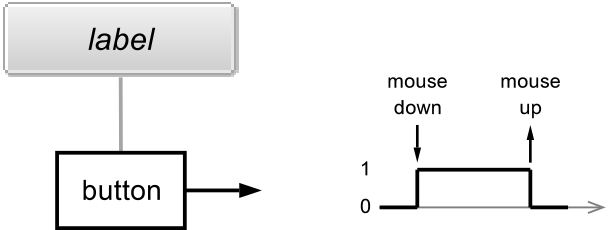
\includegraphics[scale=0.5]{illustrations/button}
\caption{User Interface Button}
\label{fig:button}
\end{figure}


\bigskip

\begin{tabular}{|l|l|}
\hline
\textbf{Syntax} & \textbf{Example} \\
\hline
\texttt{button(\farg{str})} & \texttt{button("play")}\\
\texttt{checkbox(\farg{str})} & \texttt{checkbox("mute")}\\
\texttt{vslider(\farg{str},\farg{cur},\farg{min},\farg{max},\farg{step})} & \texttt{vslider("vol",50,0,100,1)}\\
\texttt{hslider(\farg{str},\farg{cur},\farg{min},\farg{max},\farg{step})} & \texttt{hslider("vol",0.5,0,1,0.01)}\\
\texttt{nentry(\farg{str},\farg{cur},\farg{min},\farg{max},\farg{step})} & \texttt{nentry("freq",440,0,8000,1)}\\
\texttt{vgroup(\farg{str},\farg{block-diagram})} & \texttt{vgroup("reverb", \ldots)}\\
\texttt{hgroup(\farg{str},\farg{block-diagram})} & \texttt{hgroup("mixer", \ldots)}\\
\texttt{tgroup(\farg{str},\farg{block-diagram})} & \texttt{tgroup("parametric", \ldots)}\\
\texttt{vbargraph(\farg{str},\farg{min},\farg{max})} & \texttt{vbargraph("input",0,100)}\\
\texttt{hbargraph(\farg{str},\farg{min},\farg{max})} & \texttt{hbargraph("signal",0,1.0)}\\
\texttt{attach} & \texttt{attach(x, vumeter(x))}\\
\hline
\end{tabular}

\bigskip
\subsubsection{Labels}
Every user interface widget has a label (a string) that identifies it and informs the user of its purpose. There are three important mechanisms associated with labels (and coded inside the string): \textit{variable parts}, \textit{pathnames} and \textit{metadata}.

\paragraph{Variable parts.}
Labels can contain variable parts. These variable parts are indicated by the sign '\texttt{\%}' followed by the name of a variable. During compilation each label is processed in order to replace the variable parts by the value of the variable. 
For example \lstinline'par(i,8,hslider("Voice %i", 0.9, 0, 1, 0.01))' creates 8 different sliders in parallel :

\begin{lstlisting}
hslider("Voice 0", 0.9, 0, 1, 0.01),
hslider("Voice 1", 0.9, 0, 1, 0.01),
...
hslider("Voice 7", 0.9, 0, 1, 0.01).
\end{lstlisting}

while \lstinline'par(i,8,hslider("Voice", 0.9, 0, 1, 0.01))' would have created only one slider and duplicated its output 8 times.


The variable part can have an optional format digit. 
For example \lstinline'"Voice %2i"' would indicate to use two digit when inserting the value of i in the string.

An escape mechanism is provided.
If the sign \lstinline'%' is followed by itself, it will be included in the resulting string.
For example \lstinline'"feedback (%%)"' will result in \lstinline'"feedback (%)"'.

\paragraph{Pathnames.}
Thanks to horizontal, vertical and tabs groups, user interfaces have a hierarchical structure analog to a hierarchical file system. Each widget has an associated \textit{pathname} obtained by concatenating the labels of all its surrounding groups with its own label.

In the following example :
\begin{lstlisting}
hgroup("Foo",
	...
	vgroup("Faa", 
		...
		hslider("volume",...)
		...
	)
	...
)
\end{lstlisting}
the volume slider has pathname \lstinline'/h:Foo/v:Faa/volume'.

In order to give more flexibility to the design of user interfaces, it is possible to explicitly specify the absolute or relative pathname of a widget directly in its label. 

In our previous example the pathname of :
\begin{lstlisting}
	hslider("../volume",...)
\end{lstlisting}
would have been \lstinline'"/h:Foo/volume"', while the pathname of :
\begin{lstlisting}
	hslider("t:Fii/volume",...)
\end{lstlisting}
would have been : 
\lstinline'"/h:Foo/v:Faa/t:Fii/volume"'.

The grammar for labels with pathnames is the following:
% \begin{grammar}
%   <label> ::= 
%   \begin{syntdiag}
% 	<path> <name>
%   \end{syntdiag}
% \end{grammar}
% %
% \begin{grammar}
%  <path> ::= 
%   \begin{syntdiag}
% 	\begin{stack} \\ "/" \end{stack} 
% 	\begin{stack} \\ \begin{rep} <folder> "/" \end{rep} \end{stack} 
%  \end{syntdiag}
% \end{grammar}
% %
% \begin{grammar}
%  <folder> ::= 
%   \begin{syntdiag}
% 	\begin{stack}
% 		".." \\ 
% 		\begin{stack} "h:" \\ "v:" \\ "t:" \end{stack} <name>
% 	\end{stack}
%  \end{syntdiag}
% \end{grammar}

\begin{rail}
 label : path name;
 path : (| '/') (| (folder '/')+);
 folder : (".." | ("h:" | "v:" | "t:" ) name);
\end{rail}


\paragraph{Metadata}
Widget labels can contain metadata enclosed in square brackets. These metadata associate a key with a value and are used to provide additional information to the architecture file.  They are typically used to improve the look and feel of the user interface. 
The \faust code :
\begin{lstlisting}
process = *(hslider("foo [key1: val 1][key2: val 2]", 
					0, 0, 1, 0.1));
\end{lstlisting}

will produce and the corresponding C++ code :

\begin{lstlisting}
class mydsp : public dsp {
	...
	virtual void buildUserInterface(UI* interface) {
	  interface->openVerticalBox("m");
	  interface->declare(&fslider0, "key1", "val 1");
	  interface->declare(&fslider0, "key2", "val 2");
	  interface->addHorizontalSlider("foo", 
	  	&fslider0, 0.0f, 0.0f, 1.0f, 0.1f);
	  interface->closeBox();
	}
...
};
\end{lstlisting}

All the metadata are removed from the label by the compiler and 
transformed in calls to the \lstinline'UI::declare()' method. All these 
\lstinline'UI::declare()' calls will always take place before the \lstinline'UI::AddSomething()' 
call that creates the User Interface element. This allows the 
\lstinline'UI::AddSomething()'  method to make full use of the available metadata.

It is the role of the architecture file to decide what to do with these 
metadata. The \lstinline'jack-qt.cpp' architecture file for example implements the 
following :
\begin{enumerate}
\item \lstinline'"...[style:knob]..."' creates a rotating knob instead of a regular 
slider or nentry.
\item \lstinline'"...[style:led]..."' in a bargraph's label creates a small LED instead 
of a full bargraph
\item \lstinline'"...[unit:dB]..."' in a bargraph's label creates a more realistic 
bargraph with colors ranging from green to red depending of the level of 
the value
\item \lstinline'"...[unit:xx]..."' in a widget postfixes the value displayed with xx
\item \lstinline'"...[tooltip:bla bla]..."' add a tooltip to the widget
\item \lstinline'"...[osc:/address min max]..."' Open Sound Control message alias
\end{enumerate}

Moreover starting a label with a number option like in \lstinline'"[1]..."' provides
a convenient means to control the alphabetical order of the widgets.

\subsubsection{Attach}
The \lstinline'attach' primitive takes two input signals and produce one output signal which is a copy of the first input. The role of \lstinline'attach' is to force its second input signal to be compiled with the first one. From a mathematical point of view \lstinline'attach(x,y)' is equivalent to \lstinline'1*x+0*y', which is in turn equivalent to \lstinline'x', but it tells the compiler not to optimize-out \lstinline'y'.

To illustrate this role let say that we want to develop a mixer application with a vumeter for each input signals. Such vumeters can be easily coded in \faust using an envelop detector connected to a bargraph. The problem is that these envelop signals have no role in the output signals. Using \lstinline'attach(x,vumeter(x))' one can tell the compiler that when \lstinline'x' is compiled \lstinline'vumeter(x)' should also be compiled. 


